\section{Các Kiến trúc Hiện đại: ResNet, DenseNet, EfficientNet}
\label{sec:modern_architectures}

Thành công vang dội của AlexNet, VGG và GoogleNet đã xác lập một niềm tin mãnh liệt trong cộng đồng nghiên cứu: \textbf{để có hiệu năng tốt hơn, hãy làm cho mạng sâu hơn}. Triết lý đơn giản này, "càng sâu càng tốt", đã thúc đẩy một cuộc chạy đua trong việc xếp chồng thêm nhiều lớp tích chập. Tuy nhiên, các nhà nghiên cứu đã nhanh chóng vấp phải một bức tường vô hình. Khi cố gắng huấn luyện các mạng "plain" (kiến trúc xếp chồng đơn giản như VGG) với độ sâu tăng lên 30, 50, hay thậm chí 100 lớp, họ đã quan sát thấy một hiện tượng nghịch lý: hiệu năng trên cả tập huấn luyện và tập kiểm tra đều bắt đầu suy giảm.

Đây không phải là vấn đề quá khớp (overfitting), vì lỗi trên tập huấn luyện cũng tăng lên. Vấn đề nằm ở chính quá trình tối ưu hóa. Các mạng rất sâu cực kỳ khó huấn luyện, chủ yếu do hiện tượng \textbf{suy giảm/bùng nổ gradient (vanishing/exploding gradients)}. Dù ReLU đã giải quyết phần nào, nhưng trong các mạng quá sâu, gradient vẫn có thể trở nên quá nhỏ hoặc quá lớn, khiến cho việc cập nhật trọng số trở nên không hiệu quả hoặc mất ổn định. Vấn đề này được gọi chung là \textbf{vấn đề suy thoái (degradation problem)}.

Làm thế nào để xây dựng các mạng có thể hưởng lợi từ chiều sâu mà không bị suy thoái? Câu trả lời không nằm ở việc xếp chồng thêm các lớp giống hệt nhau, mà ở việc thiết kế lại chính các khối xây dựng cơ bản của mạng. Phần này sẽ khám phá ba kiến trúc mang tính đột phá đã giải quyết thành công bài toán này: ResNet, DenseNet, và EfficientNet.

\begin{center}
	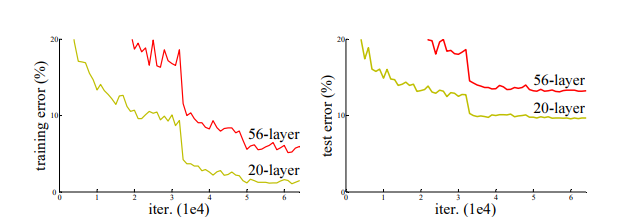
\includegraphics[width=0.7\textwidth]{images/resnet_degradation_problem.png}
	\captionof{figure}{Vấn đề suy thoái trong các mạng sâu "plain". Biểu đồ cho thấy lỗi trên tập huấn luyện và kiểm tra của một mạng 56 lớp lại cao hơn một mạng 20 lớp có cùng kiến trúc. Điều này cho thấy mạng sâu hơn không học được một hàm ánh xạ tốt bằng mạng nông hơn, dù về lý thuyết nó có khả năng đó.}
	\label{fig:resnet_degradation_problem}
\end{center}
% Keyword gợi ý: deep learning degradation problem, resnet training error graph

\subsection{ResNet (2015): Học phần dư với Kết nối tắt}
\label{subsec:resnet}
\textbf{Residual Network (ResNet)} \cite{He2016}, được giới thiệu bởi Kaiming He và các cộng sự tại Microsoft Research, là một trong những bài báo có ảnh hưởng nhất trong lịch sử học sâu. Nó đã giới thiệu một ý tưởng đơn giản nhưng thiên tài, cho phép huấn luyện thành công các mạng nơ-ron sâu hàng trăm, thậm chí hàng nghìn lớp, và đã giành chiến thắng thuyết phục tại ILSVRC 2015.

Trước ResNet, việc tăng số lớp thường dẫn đến \textbf{hiện tượng suy giảm hiệu năng (degradation problem)}: 
khi mạng càng sâu, độ chính xác trên tập huấn luyện lại giảm thay vì tăng. 
Vấn đề này không phải do overfitting, mà do khó khăn trong việc tối ưu — 
gradient bị suy yếu hoặc biến mất khiến các lớp đầu không học được. 
ResNet đã giải quyết triệt để hiện tượng này bằng cách thiết kế lại đường lan truyền thông tin 
và gradient, thay vì chỉ thay đổi cấu trúc lớp.

\subsubsection{Ý tưởng Cốt lõi: Học Ánh xạ Phần dư (Residual Learning)}
\label{subsubsec:resnet_residual_learning}
Thay vì bắt một vài lớp xếp chồng (một "block") phải học một ánh xạ cơ bản $H(\mathbf{x})$, ResNet điều chỉnh lại bài toán. Nó bắt block đó phải học một \textbf{ánh xạ phần dư (residual mapping)} $\mathcal{F}(\mathbf{x}) = H(\mathbf{x}) - \mathbf{x}$. Sau đó, output của block được tính bằng cách cộng phần dư đã học với input ban đầu:
\begin{equation}
	H(\mathbf{x}) = \mathcal{F}(\mathbf{x}) + \mathbf{x}
\end{equation}

Trên bình diện hình học, ý tưởng này tương đương với việc 
tái tham số hóa không gian hàm từ $\mathcal{H}$ sang không gian phần dư $\mathcal{F} = \mathcal{H} - \mathcal{I}$, 
trong đó $\mathcal{I}$ là phép đồng nhất. 
Nhờ đó, quá trình tối ưu hóa được “căng phẳng” (flattened optimization landscape), 
giúp quá trình học hội tụ nhanh hơn và ổn định hơn.

Phép cộng này được hiện thực hóa trong kiến trúc bằng một \textbf{"kết nối tắt" (shortcut connection} hay \textbf{skip connection)}, đi thẳng từ input của block đến sau các lớp tích chập và cộng vào output của chúng.

\begin{mdframed}[style=infobox]
	\textbf{Trực giác: Tại sao học Phần dư lại dễ hơn?}
	
	Hãy tưởng tượng trường hợp cực đoan: nếu một vài lớp trong mạng không cần làm gì cả, tức là ánh xạ tối ưu là một \textbf{ánh xạ đồng nhất (identity mapping)} $H(\mathbf{x}) = \mathbf{x}$. Đối với một mạng "plain", các lớp tích chập phải vất vả học cách để tạo ra một ma trận trọng số gần với ma trận đơn vị, một việc rất khó.
	
	Nhưng với ResNet, mọi thứ trở nên dễ dàng hơn rất nhiều. Để học một ánh xạ đồng nhất, block chỉ cần học cách làm cho $\mathcal{F}(\mathbf{x})$ tiến về 0. Việc "đẩy" các trọng số về 0 thông qua các cơ chế chính quy hóa dễ hơn rất nhiều so với việc học một ánh xạ đồng nhất phức tạp.
	
	Nói cách khác, mỗi khối ResNet chỉ cần tập trung vào việc "tinh chỉnh" hoặc "điều chỉnh" những gì đã có từ input, thay vì phải học lại toàn bộ một biểu diễn mới từ đầu.
\end{mdframed}

Luồng gradient cũng được hưởng lợi rất lớn. Trong quá trình lan truyền ngược, gradient có thể đi qua "đường tắt" một cách trực tiếp, không bị suy giảm bởi các lớp trung gian. Điều này giúp cho các lớp ở đầu mạng vẫn nhận được tín hiệu gradient mạnh mẽ, giải quyết triệt để vấn đề suy giảm gradient.

\subsubsection{Khối Xây dựng: Residual Block}
\label{subsubsec:resnet_blocks}
Kiến trúc ResNet được xây dựng từ các \textbf{Khối Phần dư (Residual Blocks)}.
\begin{description}
	\item[Basic Block:] Được sử dụng trong các mạng nông hơn như ResNet-18 và ResNet-34. Nó bao gồm hai lớp tích chập $3 \times 3$, với Batch Normalization và ReLU sau mỗi lớp. Input $\mathbf{x}$ được cộng vào output của lớp thứ hai.
	
	\item[Bottleneck Block:] Để hiệu quả hơn về mặt tính toán cho các mạng rất sâu (ResNet-50, 101, 152), khối "cổ chai" được sử dụng. Nó có cấu trúc:
	\begin{enumerate}
		\item Một lớp tích chập $1 \times 1$ để \textbf{giảm} số kênh (ví dụ: từ 256 xuống 64).
		\item Một lớp tích chập $3 \times 3$ để thực hiện xử lý không gian (trên 64 kênh).
		\item Một lớp tích chập $1 \times 1$ để \textbf{mở rộng} lại số kênh (ví dụ: từ 64 trở lại 256).
	\end{enumerate}
	Cấu trúc "giảm-xử lý-mở rộng" này giúp giảm đáng kể số lượng tham số và chi phí tính toán so với việc sử dụng hai lớp $3 \times 3$ trên số kênh lớn.
\end{description}
Nếu kích thước của $\mathbf{x}$ và $\mathcal{F}(\mathbf{x})$ không khớp nhau (do thay đổi số kênh hoặc giảm chiều không gian), kết nối tắt sẽ đi qua một lớp tích chập $1 \times 1$ (gọi là projection shortcut) để làm cho chúng khớp nhau.

\begin{table}[H]
	\centering
	\caption{Cấu hình điển hình của các phiên bản ResNet trên ImageNet}
	\label{tab:resnet_config}
	\begin{tabular}{lcccc}
		\toprule
		\textbf{Kiến trúc} & \textbf{Loại Block} & \textbf{Số Block mỗi nhóm} & \textbf{Tổng số lớp} & \textbf{Top-5 Error (\%)} \\
		\midrule
		ResNet-18 & Basic & [2, 2, 2, 2] & 18 & 7.8 \\
		ResNet-34 & Basic & [3, 4, 6, 3] & 34 & 5.7 \\
		ResNet-50 & Bottleneck & [3, 4, 6, 3] & 50 & 4.9 \\
		ResNet-101 & Bottleneck & [3, 4, 23, 3] & 101 & 4.6 \\
		ResNet-152 & Bottleneck & [3, 8, 36, 3] & 152 & 4.4 \\
		\bottomrule
	\end{tabular}
\end{table}

\begin{center}
	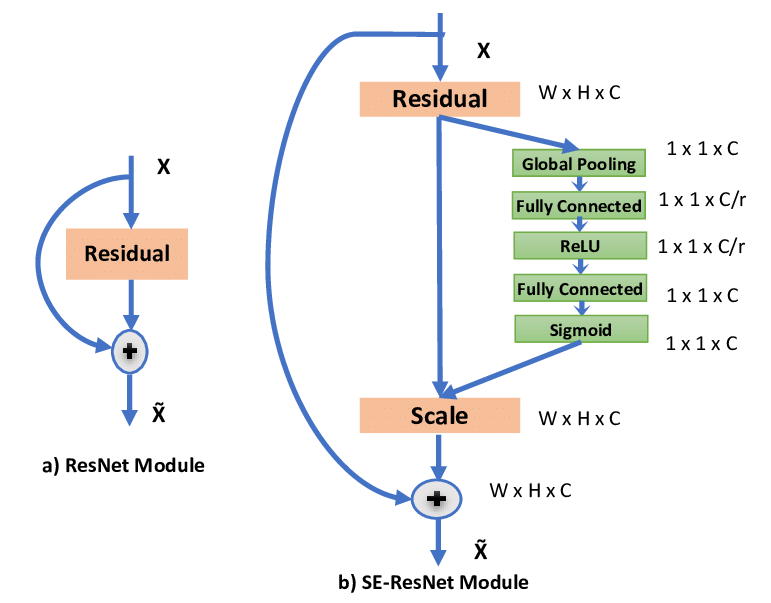
\includegraphics[width=0.9\textwidth]{images/resnet_block_vs_plain.png}
	\captionof{figure}{So sánh một khối "plain" (trái) và một Khối Phần dư (Residual Block) của ResNet (phải). Sự khác biệt duy nhất là sự có mặt của kết nối tắt (skip connection), cho phép input được cộng trực tiếp vào output.}
	\label{fig:resnet_block}
\end{center}
% Keyword gợi ý: resnet block diagram, residual block cnn

\subsubsection{Tầm ảnh hưởng}
ResNet đã đạt tỷ lệ lỗi top-5 trên ImageNet chỉ còn \textbf{3.57\%}, lần đầu tiên vượt qua hiệu năng của con người. Quan trọng hơn, nó đã cung cấp một công thức đáng tin cậy để xây dựng các mạng cực sâu. ResNet-50 và ResNet-101 nhanh chóng trở thành các kiến trúc "xương sống" mặc định cho hầu hết các tác vụ thị giác máy tính trong gần 5 năm sau đó, từ phát hiện vật thể, phân đoạn, đến ước tính tư thế.

Không chỉ dừng lại ở thị giác máy tính, ý tưởng phần dư còn được mở rộng 
sang các lĩnh vực khác như xử lý ngôn ngữ tự nhiên (Transformer Residuals), 
xử lý tín hiệu và thị giác 3D. 
ResNet cũng đặt nền móng cho hàng loạt biến thể sau này như:
\begin{itemize}
	\item \textbf{Pre-activation ResNet (2016):} Đưa BatchNorm và ReLU ra trước phép cộng phần dư, 
	giúp gradient lan truyền ổn định hơn ở các mạng cực sâu.
	\item \textbf{ResNeXt (2017):} Kết hợp ý tưởng của Inception (đa nhánh) với ResNet, 
	tăng khả năng biểu diễn mà không làm tăng đáng kể tham số.
	\item \textbf{DenseNet (2017):} Mở rộng khái niệm kết nối tắt sang kết nối “dày đặc”, 
	tức là mỗi lớp nhận input từ tất cả các lớp trước đó.
\end{itemize}


ResNet không chỉ là một bước ngoặt, mà còn là một \textit{nền tảng tư duy} 
cho các kiến trúc học sâu hiện đại. 
Nếu ResNet học phần dư giữa đầu vào và đầu ra, 
thì DenseNet — người kế nhiệm trực tiếp — sẽ tiến xa hơn bằng cách 
\textbf{kết nối tường minh tất cả các lớp với nhau}, 
biến toàn bộ mạng thành một “mạng của mạng” (network of networks).

\subsection{DenseNet (2017): Tái sử dụng Đặc trưng Tối đa}
\label{subsec:densenet}
ResNet giải quyết vấn đề luồng thông tin và gradient bằng cách cộng (summation). \textbf{Densely Connected Convolutional Network (DenseNet)} \cite{Huang2017} đề xuất một cách tiếp cận khác: thay vì cộng, hãy \textbf{nối (concatenation)}.

Khác với ResNet – nơi tín hiệu được kết hợp thông qua phép cộng, 
DenseNet sử dụng phép nối kênh để bảo toàn toàn bộ thông tin đặc trưng từ mọi lớp trước đó. 
Thay vì chỉ cho phép gradient “đi tắt” qua một đường ngắn như ResNet, 
DenseNet tạo ra một mạng lưới kết nối dày đặc, nơi mỗi lớp đều trực tiếp 
giao tiếp với tất cả các lớp trước đó. 
Điều này làm cho luồng thông tin trở nên phong phú và ổn định hơn đáng kể.

\subsubsection{Ý tưởng Cốt lõi: Kết nối Dày đặc (Dense Connectivity)}
\label{subsubsec:densenet_connectivity}
Triết lý của DenseNet là mỗi lớp nên nhận được thông tin trực tiếp từ tất cả các lớp trước đó, và truyền feature map của chính nó cho tất cả các lớp sau đó. Trong một \textbf{Dense Block}, đầu vào của lớp thứ $\ell$ là sự nối (concatenation) của các feature map của tất cả các lớp trước đó:
\begin{equation}
	\mathbf{x}_\ell = H_\ell([\mathbf{x}_0, \mathbf{x}_1, ..., \mathbf{x}_{\ell-1}])
\end{equation}
trong đó $[\mathbf{x}_0, ..., \mathbf{x}_{\ell-1}]$ là phép nối các feature map theo chiều kênh.

\begin{center}
	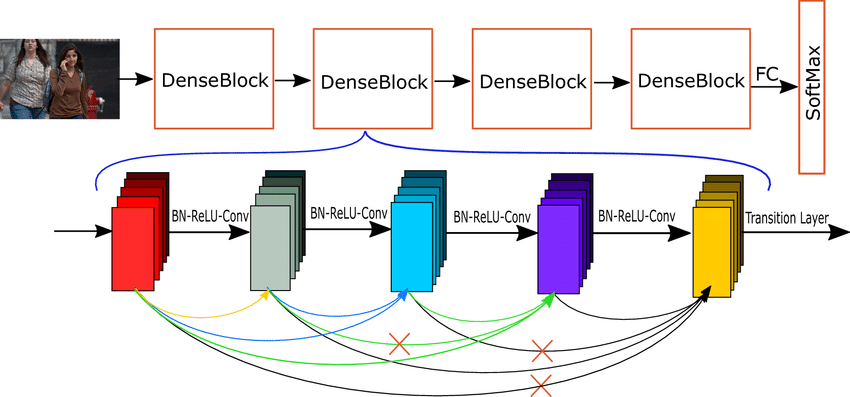
\includegraphics[width=0.5\textwidth]{images/densenet_block_diagram.png}
	\captionof{figure}{Minh họa một Dense Block với 5 lớp. Mỗi lớp nhận đầu vào là sự nối của tất cả các feature map của các lớp trước đó.}
	\label{fig:densenet_block}
\end{center}
% Keyword gợi ý: densenet block diagram, dense connectivity

Ý tưởng này mang lại nhiều lợi ích:
\begin{itemize}
	\item \textbf{Tăng cường tái sử dụng đặc trưng (Feature Reuse):} Các đặc trưng từ các lớp nông (như các cạnh) có thể được tái sử dụng trực tiếp bởi các lớp rất sâu, giúp mạng hiệu quả hơn về mặt tham số.
	\item \textbf{Giảm vấn đề suy giảm gradient:} Mỗi lớp đều nhận được tín hiệu gradient trực tiếp từ hàm mất mát, giúp việc huấn luyện trở nên dễ dàng hơn.
	\item \textbf{Hiệu quả tham số:} Vì không cần phải học lại các đặc trưng đã có, các lớp của DenseNet có thể rất "mỏng" (tạo ra ít feature map mới, một giá trị gọi là \textit{growth rate}). Kết quả là, một mạng DenseNet có thể đạt hiệu năng tương đương hoặc tốt hơn ResNet với số lượng tham số ít hơn nhiều.
\end{itemize}

Một siêu tham số quan trọng trong DenseNet là \textbf{tốc độ tăng trưởng (growth rate)}, 
ký hiệu là $k$. Đây là số lượng feature map mới mà mỗi lớp tạo ra. 
Nếu đầu vào của một Dense Block có $k_0$ kênh và block có $L$ lớp, 
thì đầu ra sẽ có $k_0 + k \times L$ kênh. 
Giá trị $k$ nhỏ (thường 12, 24 hoặc 32) giúp mạng vẫn gọn nhẹ mặc dù có nhiều kết nối.

\subsubsection{Kiến trúc và các Lớp Chuyển tiếp (Transition Layers)}
Kiến trúc DenseNet bao gồm nhiều Dense Block. Một vấn đề của việc nối liên tục là số kênh sẽ tăng lên rất nhanh. Để kiểm soát điều này, giữa các Dense Block là các \textbf{Lớp Chuyển tiếp (Transition Layers)}, có nhiệm vụ:
\begin{enumerate}
	\item Sử dụng một lớp tích chập $1 \times 1$ để nén số kênh (ví dụ, giảm một nửa).
	\item Sử dụng một lớp Average Pooling $2 \times 2$ để giảm chiều không gian.
\end{enumerate}

\subsection{EfficientNet (2019): Cân bằng Kiến trúc với Compound Scaling}
\label{subsec:efficientnet}
Vào năm 2019, cuộc đua về chiều sâu đã dần bão hòa. Các nhà nghiên cứu bắt đầu tìm kiếm sự cân bằng giữa độ chính xác, chi phí tính toán (FLOPs), và số lượng tham số. ResNet có thể được làm "rộng" hơn (tăng số kênh) hoặc huấn luyện với ảnh có độ phân giải cao hơn để cải thiện hiệu năng, nhưng việc tinh chỉnh các yếu tố này (độ sâu, độ rộng, độ phân giải) thường được thực hiện một cách thủ công và không hiệu quả.

\textbf{EfficientNet} \cite{Tan2019}, từ Google AI, đã giới thiệu một nguyên lý mới để mở rộng quy mô mạng một cách có hệ thống: \textbf{Compound Scaling}.

\subsubsection{Ý tưởng Cốt lõi: Mở rộng Quy mô Hỗn hợp (Compound Scaling)}
\label{subsubsec:efficientnet_scaling}
Ý tưởng chính là thay vì chỉ tăng một trong ba chiều của mạng (độ sâu $d$, độ rộng $w$, độ phân giải $r$), chúng ta nên tăng cả ba một cách cân bằng và đồng thời. EfficientNet đề xuất một hệ số hỗn hợp $\phi$ để điều khiển việc này:
\begin{align}
	\text{depth: }\& d = \alpha^\phi \\
	\text{width: }\& w = \beta^\phi \\
	\text{resolution: }\& r = \gamma^\phi
\end{align}
với các hằng số $\alpha, \beta, \gamma$ được tìm ra thông qua một cuộc tìm kiếm lưới nhỏ trên một mô hình cơ sở. Các hằng số này bị ràng buộc bởi $\alpha \cdot \beta^2 \cdot \gamma^2 \approx 2$, sao cho việc tăng $\phi$ lên 1 sẽ làm tăng tổng FLOPs lên khoảng $2^\phi$ lần.

\subsubsection{Kiến trúc và Kết quả}
EfficientNet bắt đầu với một kiến trúc cơ sở hiệu quả là \textbf{EfficientNet-B0}, được tìm ra thông qua Tìm kiếm Kiến trúc Nơ-ron (Neural Architecture Search - NAS). Kiến trúc này sử dụng các khối \textbf{MBConv} (từ MobileNetV2) kết hợp với cơ chế \textbf{Squeeze-and-Excitation (SE)} để tăng cường đặc trưng.

\paragraph{Khối MBConv và Squeeze-and-Excitation (SE):}
Khối \textbf{MBConv} là phiên bản mở rộng của Inverted Residual Block trong MobileNetV2, 
gồm ba giai đoạn chính:
\begin{enumerate}
	\item \textbf{Expansion:} Một lớp tích chập $1 \times 1$ để mở rộng số kênh đầu vào lên hệ số $t$ (thường $t=6$).
	\item \textbf{Depthwise Convolution:} Tích chập theo từng kênh riêng biệt, giúp giảm chi phí tính toán.
	\item \textbf{Projection:} Một lớp $1 \times 1$ khác để nén số kênh về lại kích thước ban đầu.
\end{enumerate}
Sau khối này, cơ chế \textbf{Squeeze-and-Excitation (SE)} được áp dụng để tái cân bằng các kênh:
\begin{itemize}
	\item \textbf{Squeeze:} Nén không gian bằng Global Average Pooling.
	\item \textbf{Excitation:} Học trọng số cho từng kênh qua hai lớp fully connected nhỏ.
\end{itemize}

\begin{center}
	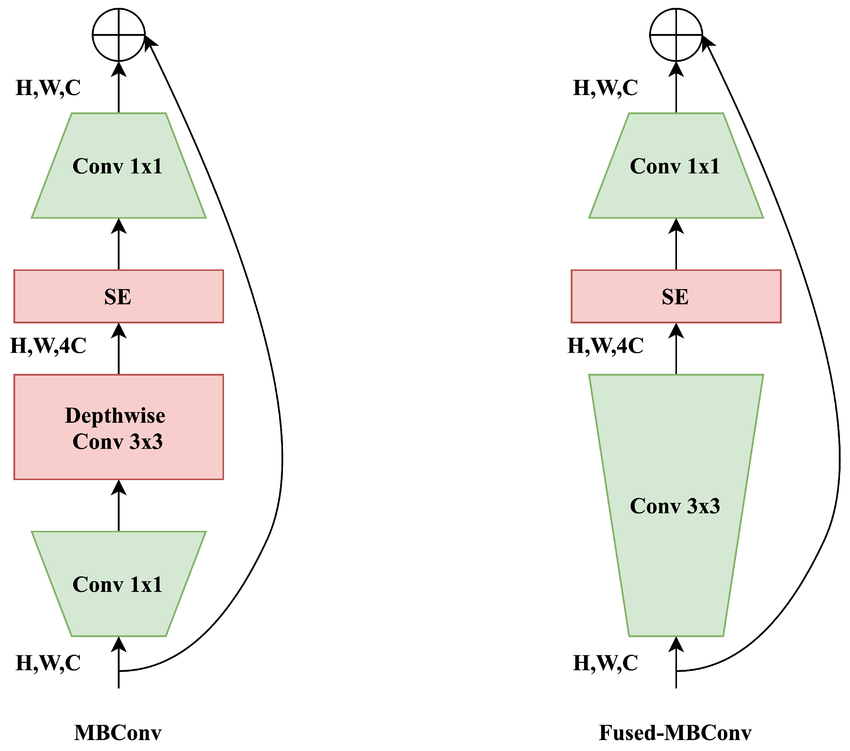
\includegraphics[width=0.8\textwidth]{images/efficientnet_mbconv.png}
	\captionof{figure}{Cấu trúc của khối MBConv với cơ chế SE. 
		Các kết nối tắt (skip connections) được sử dụng khi kích thước đầu vào và đầu ra trùng khớp.}
	\label{fig:efficientne}
\end{center}
Sau đó, bằng cách tăng hệ số $\phi$ từ 1 đến 7, họ tạo ra một họ các mô hình từ EfficientNet-B1 đến B7. Kết quả thật ấn tượng:
\begin{itemize}
	\item EfficientNet-B0 đạt hiệu năng tương đương ResNet-50 nhưng với số lượng tham số ít hơn gần 5 lần.
	\item EfficientNet-B7 đạt được state-of-the-art mới trên ImageNet với độ chính xác và hiệu quả vượt trội so với tất cả các mô hình trước đó.
\end{itemize}

\begin{table}[H]
	\centering
	\caption{Các biến thể EfficientNet trên ImageNet}
	\label{tab:efficientnet_versions}
	\begin{tabular}{lcccc}
		\toprule
		\textbf{Phiên bản} & \textbf{Độ sâu ($d$)} & \textbf{Độ rộng ($w$)} & \textbf{Độ phân giải ($r$)} & \textbf{Top-1 Accuracy (\%)} \\
		\midrule
		B0 & 1.0× & 1.0× & 224 & 77.1 \\
		B1 & 1.1× & 1.0× & 240 & 79.1 \\
		B2 & 1.2× & 1.1× & 260 & 80.1 \\
		B3 & 1.4× & 1.2× & 300 & 81.6 \\
		B4 & 1.8× & 1.4× & 380 & 83.0 \\
		B5 & 2.2× & 1.6× & 456 & 83.6 \\
		B6 & 2.6× & 1.8× & 528 & 84.0 \\
		B7 & 3.1× & 2.0× & 600 & 84.4 \\
		\bottomrule
	\end{tabular}
\end{table}

\begin{center}
	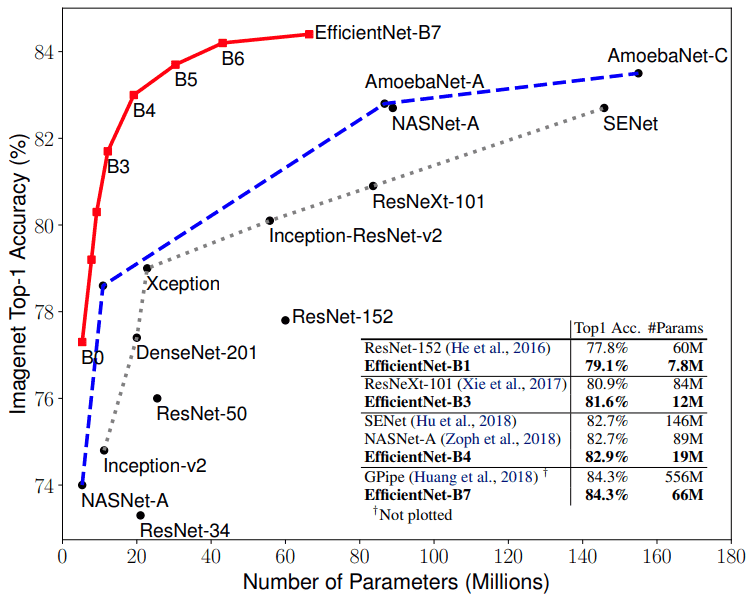
\includegraphics[width=0.8\textwidth]{images/efficientnet_accuracy_vs_flops.png}
	\captionof{figure}{So sánh hiệu năng (độ chính xác trên ImageNet) và chi phí tính toán (FLOPs). Họ mô hình EfficientNet (đường màu đỏ) đãđỏ thiết lập một biên Pareto mới, cho thấy hiệu quả vượt trội so với các kiến trúc trước đó như ResNet và DenseNet.}
	\label{fig:efficientnet_flops}
\end{center}
% Keyword gợi ý: efficientnet accuracy flops, model scaling compound

EfficientNet không chỉ tạo ra một họ mô hình mạnh mẽ, mà còn giới thiệu một phương pháp luận mới về việc thiết kế và mở rộng quy mô mạng. Nó đánh dấu sự chuyển dịch từ việc thiết kế thủ công, dựa trên kinh nghiệm, sang việc tối ưu hóa kiến trúc dựa trên các nguyên tắc toán học và tìm kiếm tự động.

\section*{Tài liệu tham khảo}
\begin{itemize}
	\item[1] He, K., Zhang, X., Ren, S.,\& Sun, J. (2016). Deep residual learning for image recognition. In \textit{Proceedings of the IEEE conference on computer vision and pattern recognition (CVPR)}. (Paper gốc giới thiệu ResNet, một trong những bài báo có ảnh hưởng nhất trong lịch sử học sâu).
	\item[2] Huang, G., Liu, Z., Van Der Maaten, L.,\& Weinberger, K. Q. (2017). Densely connected convolutional networks. In \textit{Proceedings of the IEEE conference on computer vision and pattern recognition (CVPR)}. (Paper gốc giới thiệu DenseNet và ý tưởng kết nối dày đặc).
	\item[3] Tan, M.,\& Le, Q. V. (2019). Efficientnet: Rethinking model scaling for convolutional neural networks. In \textit{International Conference on Machine Learning (ICML)}. (Paper gốc giới thiệu EfficientNet và nguyên lý Compound Scaling).
	\item[4] Simonyan, K.,\& Zisserman, A. (2014). Very deep convolutional networks for large-scale image recognition. \textit{arXiv preprint arXiv:1409.1556}. (Paper về VGG, cung cấp bối cảnh về các mạng "plain" sâu và các vấn đề của chúng).
	\item[5] Howard, A. G., Zhu, M., Chen, B., Kalenichenko, D., Wang, W., Weyand, T., ...\& Adam, H. (2017). Mobilenets: Efficient convolutional neural networks for mobile vision applications. \textit{arXiv preprint arXiv:1704.04861}. (Paper giới thiệu MobileNet, nền tảng cho khối MBConv được sử dụng trong EfficientNet).
	\item[6] Hu, J., Shen, L.,\& Sun, G. (2018). Squeeze-and-excitation networks. In \textit{Proceedings of the IEEE conference on computer vision and pattern recognition (CVPR)}. (Paper giới thiệu khối Squeeze-and-Excitation, một thành phần quan trọng giúp tăng hiệu quả của EfficientNet).
\end{itemize}